% Options for packages loaded elsewhere
\PassOptionsToPackage{unicode}{hyperref}
\PassOptionsToPackage{hyphens}{url}
%
\documentclass[
  11pt,
  a4paper,
]{article}
\usepackage{amsmath,amssymb}
\usepackage{lmodern}
\usepackage{iftex}
\ifPDFTeX
  \usepackage[T1]{fontenc}
  \usepackage[utf8]{inputenc}
  \usepackage{textcomp} % provide euro and other symbols
\else % if luatex or xetex
  \usepackage{unicode-math}
  \defaultfontfeatures{Scale=MatchLowercase}
  \defaultfontfeatures[\rmfamily]{Ligatures=TeX,Scale=1}
  \setmainfont[]{roboto}
\fi
% Use upquote if available, for straight quotes in verbatim environments
\IfFileExists{upquote.sty}{\usepackage{upquote}}{}
\IfFileExists{microtype.sty}{% use microtype if available
  \usepackage[]{microtype}
  \UseMicrotypeSet[protrusion]{basicmath} % disable protrusion for tt fonts
}{}
\makeatletter
\@ifundefined{KOMAClassName}{% if non-KOMA class
  \IfFileExists{parskip.sty}{%
    \usepackage{parskip}
  }{% else
    \setlength{\parindent}{0pt}
    \setlength{\parskip}{6pt plus 2pt minus 1pt}}
}{% if KOMA class
  \KOMAoptions{parskip=half}}
\makeatother
\usepackage{xcolor}
\usepackage[margin=2.5cm]{geometry}
\usepackage{longtable,booktabs,array}
\usepackage{calc} % for calculating minipage widths
% Correct order of tables after \paragraph or \subparagraph
\usepackage{etoolbox}
\makeatletter
\patchcmd\longtable{\par}{\if@noskipsec\mbox{}\fi\par}{}{}
\makeatother
% Allow footnotes in longtable head/foot
\IfFileExists{footnotehyper.sty}{\usepackage{footnotehyper}}{\usepackage{footnote}}
\makesavenoteenv{longtable}
\usepackage{graphicx}
\makeatletter
\def\maxwidth{\ifdim\Gin@nat@width>\linewidth\linewidth\else\Gin@nat@width\fi}
\def\maxheight{\ifdim\Gin@nat@height>\textheight\textheight\else\Gin@nat@height\fi}
\makeatother
% Scale images if necessary, so that they will not overflow the page
% margins by default, and it is still possible to overwrite the defaults
% using explicit options in \includegraphics[width, height, ...]{}
\setkeys{Gin}{width=\maxwidth,height=\maxheight,keepaspectratio}
% Set default figure placement to htbp
\makeatletter
\def\fps@figure{htbp}
\makeatother
\setlength{\emergencystretch}{3em} % prevent overfull lines
\providecommand{\tightlist}{%
  \setlength{\itemsep}{0pt}\setlength{\parskip}{0pt}}
\setcounter{secnumdepth}{-\maxdimen} % remove section numbering
\newlength{\cslhangindent}
\setlength{\cslhangindent}{1.5em}
\newlength{\csllabelwidth}
\setlength{\csllabelwidth}{3em}
\newlength{\cslentryspacingunit} % times entry-spacing
\setlength{\cslentryspacingunit}{\parskip}
\newenvironment{CSLReferences}[2] % #1 hanging-ident, #2 entry spacing
 {% don't indent paragraphs
  \setlength{\parindent}{0pt}
  % turn on hanging indent if param 1 is 1
  \ifodd #1
  \let\oldpar\par
  \def\par{\hangindent=\cslhangindent\oldpar}
  \fi
  % set entry spacing
  \setlength{\parskip}{#2\cslentryspacingunit}
 }%
 {}
\usepackage{calc}
\newcommand{\CSLBlock}[1]{#1\hfill\break}
\newcommand{\CSLLeftMargin}[1]{\parbox[t]{\csllabelwidth}{#1}}
\newcommand{\CSLRightInline}[1]{\parbox[t]{\linewidth - \csllabelwidth}{#1}\break}
\newcommand{\CSLIndent}[1]{\hspace{\cslhangindent}#1}
\usepackage{lineno}
\usepackage{authblk}
\usepackage{lipsum} \usepackage{float} \floatplacement{figure}{H} \usepackage[sfdefault]{roboto} \usepackage[T1]{fontenc} 

%command for the package lineno to put line numbers in the manuscript
\linenumbers

% make it double spaced
\usepackage{setspace}
\doublespacing

%authors
\author[1,*]{Sarah P. Flanagan}
\author[2]{Suzanne H. Alonzo}
\affil[1]{\footnotesize School of Biological Sciences, University of Canterbury}
\affil[2]{\footnotesize Department of Ecology and Evolutionary Biology, University of California Santa Cruz}
\affil[*]{Corresponding author: spflanagan.phd@gmail.com}
\usepackage{booktabs}
\usepackage{longtable}
\usepackage{array}
\usepackage{multirow}
\usepackage{wrapfig}
\usepackage{float}
\usepackage{colortbl}
\usepackage{pdflscape}
\usepackage{tabu}
\usepackage{threeparttable}
\usepackage{threeparttablex}
\usepackage[normalem]{ulem}
\usepackage{makecell}
\usepackage{xcolor}
\ifLuaTeX
  \usepackage{selnolig}  % disable illegal ligatures
\fi
\IfFileExists{bookmark.sty}{\usepackage{bookmark}}{\usepackage{hyperref}}
\IfFileExists{xurl.sty}{\usepackage{xurl}}{} % add URL line breaks if available
\urlstyle{same} % disable monospaced font for URLs
\hypersetup{
  pdftitle={Supergenes are not necessary to explain the maintenance of complex alternative phenotypes},
  hidelinks,
  pdfcreator={LaTeX via pandoc}}

\title{Supergenes are not necessary to explain the maintenance of complex alternative phenotypes}
\date{\vspace{-2.5em}}

\begin{document}
\maketitle
\begin{abstract}
Evolutionary biology aims to explain the diversity seen in nature. Evolutionary theory provides frameworks to understand how simple polymorphisms or continuous variation are maintained, but phenotypes inherited as discrete suites of quantitative traits are difficult to fit into this framework. Supergenes have been proposed as a solution to this problem -- if causal genes are co-located, they can be inherited as if a single gene, thus bridging the gap between simple polymorphisms and continuous traits. We develop models to ask: how critical are supergenes for maintaining phenotypic diversity? In our simplest model, without explicit genetic architectures, three alternative reproductive morphs are maintained in many of the parameter combinations we evaluated. With these same parameters, models with demographic stochasticity, recombination, and mutation maintained only two of these three morphs, with stochasticity determining which ones. With explicit genetic architectures, regardless of whether causal loci were co-located in a supergene or distributed randomly, this stochasticity was reduced. Even when phenotypic variation was lost, genetic diversity was maintained. Altogether, categorical traits with polygenic bases exhibited similar evolutionary dynamics to those determined by supergenes. Our work suggests that supergenes are not the only answer to the puzzle of how discrete phenotypic variation is maintained. ¶ \par ¶ \textbf{Keywords:} genome-wide genetic diversity, alternative mating tactics, frequency dependent selection, supergene, alternative reproductive tactics, genetic architecture
\end{abstract}

\hypertarget{introduction}{%
\section{Introduction}\label{introduction}}

A wide variety of animals exhibit sex-specific morphs that are generally
associated with different discrete ways of maximizing reproductive
success, which are often referred to as alternative reproductive tactics
{[}1{]}. These stable
polymorphisms are typically maintained in populations through negative
frequency-dependent selection (e.g., female morphs in damselflies
{[}2{]}; Gouldian finches
{[}3{]}), the interaction
of frequency-dependent and density-dependent factors (e.g.,
side-blotched lizards {[}4{]}), and fluctuating
selection pressures enabling the partitioning of reproductive success
over time (e.g., the feminized dwarf spider morph mates earlier, whereas
the alternative morph is able to mate with previously-mated females
later in the season {[}5{]}).
When these tactics are fixed within an individual throughout its
lifetime, an individual's tactic often has a large genetic component
(e.g., dwarf spiders, side-blotched lizards, ruffs; examples reviewed in
{[}1,6{]}). The maintenance of fixed tactics
have been modelled using explicitly or implicitly simple genetic
architectures of one or two genetic loci
{[}4,7--13{]}. Given that morphs are suites of
traits inherited together, some authors have used verbal models to
explore the importance of correlational selection and its associated
formation of genetic correlations and linkage disequilibrium across loci
{[}14{]}. While these relatively
simple genetic models do capture the evolutionary dynamics of some
empirical examples {[}7,15{]}, genomic data has accumulated
for a number of species suggesting that categorical traits might in fact
be underpinned by numerous quantitative genetic loci
{[}16,17{]}.

Consistent with other work suggesting that traits critical to
reproductive fitness are determined by the additive contributions of
many loci throughout the genome {[}17,18{]}, several alternative
reproductive tactics are associated with many genetic variants
throughout the genome which contribute primarily additively to the
phenotypes {[}16{]} -- implying that although
the tactics might be discrete and inherited in an apparently Mendelian
fashion, their genetic basis is much more complex and multivariate. A
particularly intriguing result is that structural variants have
aggregated multiple variants contributing to the tactics into a
`supergene' in at least three species with alternative reproductive
tactics: the ruff {[}19,20{]}, white-throated sparrow
{[}21{]}, and dwarf spiders
{[}5{]}. Supergenes have also
been linked to sex-specific traits important to reproduction such as
sperm morphology {[}22,23{]}, head colour
{[}24{]}, and sex-specific migratory
behaviours {[}25{]}. The potential
for supergenes to underpin sexually dimorphic polyphenisms is
intriguing, as it could explain the apparent mis-match between simple
single-locus population genetic models and the fact that these
reproductive tactics are suites of complex traits
{[}7{]}. Supergenes, with their reduced
recombination between variants, also provide a mechanism for individuals
with largely similar genomic information to harbour fixed genetic
variation without requiring differential gene expression. Examples where
supergenes apparently underpin sexually dimorphic phenotypes tend to
involve multiple morphs of one sex, usually males. All known examples of
alternative morphs determined by supergenes include a female-mimic
morph, including ruffs {[}19,20{]}, dwarf spiders
{[}5{]}, and white-throated
sparrows {[}21{]}. In the ruffs, a
third male morph exists, with an intermediate phenotype between the
dominant or `classic' male morph and the female-mimic
{[}19,20{]}. In some cases, a heterozygous
genotype is lethal (e.g., ruffs {[}19,20{]}), but not in others (e.g.,
dwarf spiders {[}5{]}). In the
white-throated sparrow and the ruff, these structural variants are
successful in coding for these variable phenotypes because they include
androgen receptors {[}26{]}-- the white-throated
sparrow supergene contains the estrogen receptor gene which directly
influences the aggressive aspects of the dominant male phenotype
{[}27{]}.

An open question is: to what extent do supergenes facilitate the
maintenance of multiple morphs versus the evolution of multiple morphs
facilitating the evolution of supergenes? This question is difficult to
address empirically, but is important for understanding the genetic
mechanisms underpinning adaptive genetic variation. For example, if a
supergene exists and a mutation arises within it that affects the morph
traits, the genetic variation within the supergene itself could have
eroded due to relaxation of selection and reduced recombination. As
such, only the mutation would be likely to show significant genetic
variation -- this could make a supergene with functional effects
difficult to detect empirically. This is especially true in cases such
as the white-throated sparrow, in which the gene with a major effect is
an estrogen receptor {[}27{]},
which likely affects the expression of many genes. Furthermore, it is
currently unknown to what extent genetic architectures -- and the
constraints inherit to them -- impact the dynamics of the frequency- and
density-dependent mechanisms that maintain simple cases of genetic
variation in populations.

An additional challenge arises from limitations in the empirical data
that can be used to identify genetic architectures of these traits and
uncover the mechanisms governing their evolution. The majority of
examples involved researchers first generating a high quality reference
genome and subsequently performing whole genome resequencing of
individuals of each morph and sex to identify variants within
populations that are associated with the phenotypic tactics
{[}5,16,19--22,27,28{]}. Alternative approaches
involve linkage mapping {[}29{]} or the
investigation of differential gene expression between morphs
{[}30--32{]}. These methods have proven
successful in some cases, although for many other types of traits the
ability to detect causal variants is generally limited
{[}33--35{]}. Regardless, despite the
potential ability to uncover the most important evolutionary processes
in the evolution of these traits using genomic data
{[}36--38{]}, the power might be
substantially limited in real-world samples
{[}39,40{]}. In part, this limitation is
due to lacking a predictive understanding of how different genetic
architectures can influence evolutionary dynamics of polygenic traits.

To tackle these problems, we use models to test how different genetic
architectures affect the maintenance of multiple male reproductive
morphs. We focus on first identifying key reproductive parameters that
influence the maintenance or loss of morphs using an analytical haploid
model. Using a simulation model, we test whether different types of
diploid genetic architectures (single locus, polygenic, and polygenic
supergene) change the presence of and relative frequencies of morphs
that are maintained. We then use the output of these simulation models
to test the accuracy and ability of current empirical methods to
identify the causal genetic variants underlying the alternative
reproductive tactics.

\hypertarget{methods}{%
\section{Methods}\label{methods}}

Our model considers a biological scenario in which males can display to
attract females and provide obligate male parental care. To allow us to
answer our questions about supergenes facilitating multiple morphs, we
consider two two independent traits, courtship and parental care, both
of which are expressed only in males. We assume that all females in the
population prefer males with the courting trait, but females do not know
when choosing a male whether that male will also provide care. Males who
do not court can only reproduce by sneaking, and males who display but
do not provide any parental care will not produce viable offspring.
Thus, our model has four potential tactics: courter/parents (CP);
courter/non-parents (CN); non-courters/parents (NP); or
non-courters/non-parents (NN). Our model assumes non-overlapping
generations and no environmental effects on traits. While this model
does not directly apply to all examples of alternative reproductive
tactics, it is biologically reasonable and common even if not
universally true. We expect that this model can be generalized to
species in which one sex (but not the other) has two fixed traits that
affect mating success and the survival of their offspring.

To test the importance of genetic architecture in male morphs, we
implemented three models. First, we developed an analytical model that
reflects haploid inheritance of a single locus that encodes morphs. This
model did not include recombination or mutation. Second, we used a
stochastic individual-based model with two diploid loci, one for each
trait (courting and parenting), that incorporated recombination,
mutation, and demographic stochasticity. Finally, we expanded the
stochastic model to incorporate polygenic inheritance of the two traits,
with two different explicit physical genetic architectures: quantitative
trait loci (QTLs) distributed at random throughout a genome including
non-coding loci and a supergene architecture, where QTLs were co-located
in a non-recombining region of a single chromosome. We assumed all QTLs
were autosomal. Each allele at a QTL was assigned a randomly-drawn
phenotypic effect, and an individual's quantitative phenotypic value was
determined by the sum of all their allelic effects (i.e., traits were
entirely additive). In these additive, polygenic models, male traits
were determined by a threshold function. The value of the threshold was
constant for each iteration of the model, and was initialized as the
mean phenotypic value at generation 0, prior to any model iterations. In
all cases of the individual-based models, Sex was assigned instead by a
draw from a binomial distribution with a probability of 0.5 of being
female.

In all three models, each generation has five distinct phases: (1) mate
choice; (2) fertilization; (3) parental care; (4) viability selection;
and (5) maturation to adulthood (Fig. \ref{fig:modelDiagram}). We will
describe each of these phases and highlight differences between the
models when appropriate.

\begin{figure}[H]
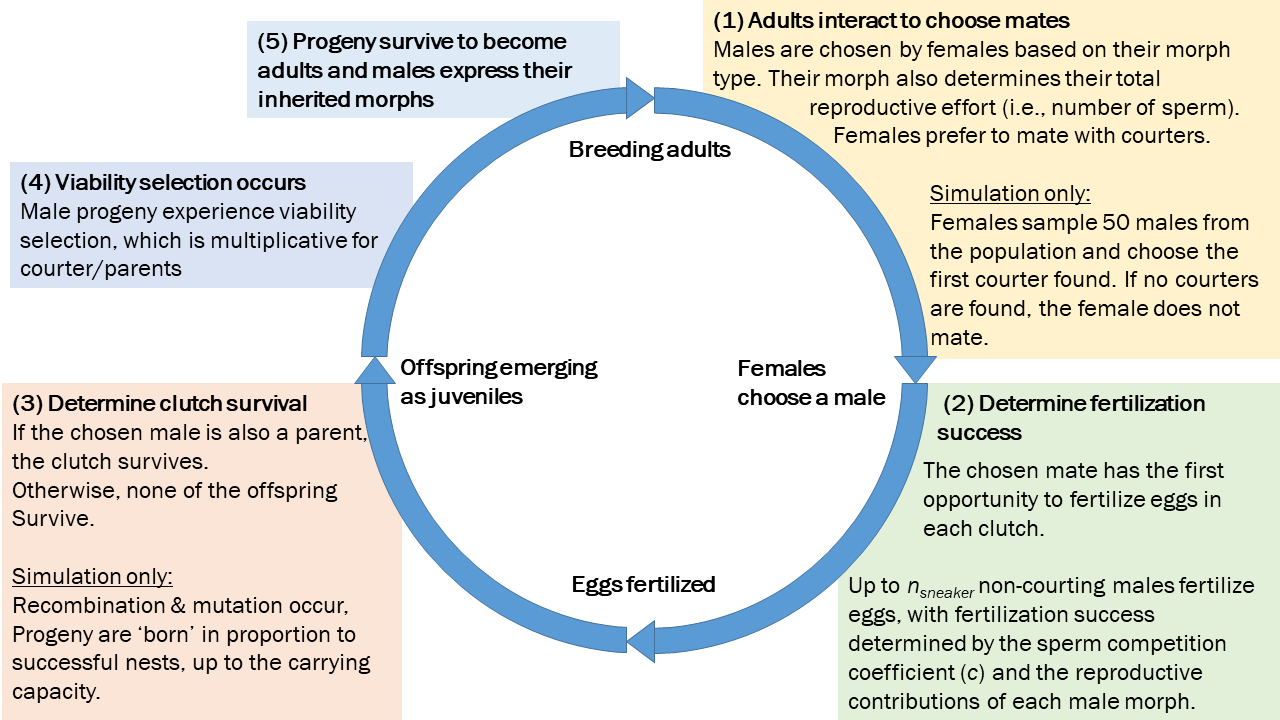
\includegraphics[width=1\linewidth,]{../figs/lifecycle_biology} \caption{Diagram of the biological life cycle modelled in both the analytical model and the simulation model. The model has five phases, starting with (1) Adults interact to find mates. Differences between the models are articulated in the diagram.}\label{fig:modelDiagram}
\end{figure}

\hypertarget{stage-1-mate-choice}{%
\subsection{Stage 1: Mate choice}\label{stage-1-mate-choice}}

In the mate choice phase of the model, we assumed females always
preferred to mate with males displaying the courtship trait and did not
mate with non-courting males. If a female decided to mate with a male,
he received all of her eggs to care for.

In the analytical model, this mate choice phase determined to total
number of clutches in the population, \(n\). The general calculation for
the number of clutches is:

\[
n=w_s(N_m f_{CP} + N_m f_{CN}) + (1-w_s)(N_m f_{NP} + N_m f_{NN}), 
\]

where \(w_s\) specified the probability a female chose a courting male (CP
or CN), \(N_m\) was the number of males in the population, the \(f\) terms
represented the frequency of each morph. To match our model assumptions,
\(w_s=1\), so \(n\) simplified to \(w_s(N_m f_{CP} + N_m f_{CN})\).

The simulation model incorporated stochasticity at this stage of the
model. Females searched through a set number of males and chose the
first attractive male (i.e., the first courting male she encountered).
If a female did not find an acceptable mate, she did not mate.

\hypertarget{stage-2-fertilization}{%
\subsection{Stage 2: Fertilization}\label{stage-2-fertilization}}

A chosen male was not guaranteed paternity of an entire brood, because
non-courting males were able to fertilize a proportion of the eggs. The
chosen parent had first-male fertilization advantage. The consequence of
this scenario is that the only mechanism by which non-courters can
produce offspring is through sneak fertilizations. Specifically, we
modelled sneaking by specifying a total number of sneakers, \(n_{sneak}\),
that could fertilise via sneaking in each clutch, and each sneaker could
contribute up to their individual reproductive allocation (where
\(r_{NN} = r_{NP}\)) offset by the sperm competition coefficient (\(c\)). We
explored the effect of different values of these parameters in the
analytical model, but for all simulation models analysed here,
\(n_{sneak}=3\) and \(c=0.5\). We also assumed inherent `reproductive
allocations',\(r_M\) (where \(M\) designated the morph and contained
\(\{CP, CN, NP, NN\}\)), for each morph, which sets a ceiling on the
number of offspring any male can sire.

In the analytical model, we modelled the fertilisation success for
morphs by considering their fertilisation success in clutches laid by
the females who chose them, \(e_{o_M} = f_M N_m r_M w_{s_M}\) (which will
only be non-zero for courting morphs). We specified the maximum number
of possible fertilizations arising from sneaking for a given
non-courting morph was \(N_s = n c n_{sneakers} r_{NN}\). If the number of
fertilizations arising from sneaking was smaller than the morph's
potential population-level reproductive effort (i.e, if
\(N_s < f_M N_m r_M\)), the number of eggs fertilized through sneaking for
that morph was the difference between \(N_s\) and \(f_M N_m r_M\), truncated
at zero. Otherwise, the number of eggs fertilized through sneaking was
\(f_M N_m r_M\).

In the simulation model, we incorporated recombination and mutation
during the fertilisation process. Recombination occurred independently
on chromosomes inherited from the mother and the father. The number of
recombination events for a given chromosome was determined by drawing
from a Poisson distribution with the recombination rate as the mean,
which we set to 0.2. For each recombination event, breakpoints were
chosen by randomly drawing from the total number of markers on a
chromosome. These breakpoints defined the segments of the chromosome
that experienced recombination, and each segment was randomly chosen to
be assigned the genotypes and effects from the parents' maternal or
paternal chromosome. When the genetic architecture was that of a
supergene, if the breakpoints fell within the region containing the
aggregated QTLs for the traits, the offspring was considered not viable,
mimicking suppressed recombination as observed in empirical examples
(e.g., ruffs {[}19,20{]}).

After recombination, mutation occurred at a rate of \(\mu\) at each locus.
For a given individual, the number of mutations introduced was
determined as \(2\mu n_{SNPs} n_{chrom}\), where \(n_{SNPs}\) was the number
of SNPs and \(n_{chrom}\) was the number of chromosomes in the simulation.
The location of each mutation was randomly selected and the allele at
that location was randomly chosen from the set of existing alleles. The
mutation also affected the phenotypic effects of QTLs by altering the
original effect by a value drawn from a normal distribution with a mean
of 0 and a standard deviation of \(\sigma_\mu\). Finally, offspring were
also randomly assigned a sex.

\hypertarget{stage-3-parental-care}{%
\subsection{Stage 3: Parental care}\label{stage-3-parental-care}}

We assumed for simplicity that males with the parental care trait have
100\% offspring survival while males without the parental care trait have
0\% survival, independent of the male's courtship trait. This was
straightforward to model in the simulations: after the males were
assigned their paternity shares (during fertilisation), the clutch
survived if the chosen male was also a parent. Because of this
assumption, and those in Stage 1, the courter/non-parent morph never
produced viable offspring.

In the baseline model, we modelled this by defining the selection
coefficient for clutch survival, \(w_{n_M}\), which determined the success
of each morph's clutch, assuming the morph was chosen by a female:
\(o_{o_M} = e_{o_M} w_{n_M}\). To match our model assumptions,
\(w_{n_CP} = w_{NP} = 1\) and \(w_{n_CN} = w_{NN} = 0\). We also calculated
the number of surviving offspring from sneaking as:

\[
o_{s_M} = e_{s_M} \frac{\Sigma{o_{o_M}}}{\Sigma{e_{o_M}}}.
\]

Because we assumed obligate parental care, the fraction was either 1 or
0, depending on whether the morph associated with the clutch had the
parental care trait. Each morph's total number of offspring produced
(\(o_M\)) was the sum of \(o_{o_M}\) and \(o_{s_M}\).

\hypertarget{stage-4-viability-selection}{%
\subsection{Stage 4: Viability selection}\label{stage-4-viability-selection}}

We assumed viability selection only affects male offspring, through a
trade-off between courting and parental care. In the baseline model, we
multiplied the viability selection coefficient (\({w_v}_M\)) by the
surviving number of offspring per morph (\(o_M\)), to determine the number
of surviving juveniles per morph: \(j_M = o_M w_{v_M}\). In the simulation
model, we calculated a survival probability for each male offspring, as
\(e^{\frac{-(morph - \theta)(morph - \theta)}{2\omega_v}}\), where
\(\omega_v\) represents the strength of viability selection, \(morph\) is 1
for courters and parents and 0 for non-courters and non-parents, and
\(\theta = 0\) (i.e., selection favours the non-courters and non-parents).
For each individual, a random value between 0 and 1 was drawn from a
uniform distribution; if the number was larger than his survival
probability, that individual did not survive to adulthood. In both
models, viability selection acted multiplicatively on courter/parents.

\hypertarget{stage-5-maturation-to-adulthood}{%
\subsection{Stage 5: Maturation to adulthood}\label{stage-5-maturation-to-adulthood}}

In the baseline model, the final stage in the life cycle was calculating
the frequency of each morph in the next generation by dividing the
surviving number of juveniles per morph after viability selection
(\(j_M\)) by the sum of all surviving juveniles:
\(f_M = \frac{j_M}{\Sigma_{i=1}^4{j_i}}\).

In the simulation model, the total number of surviving offspring in the
population depended on the proportion of population reproductive success
achieved by each individual male and female (i.e., each generation, the
number of offspring created was equal to the carrying capacity). If the
number of surviving offspring was larger than the carrying capacity,
offspring were randomly selected to become adults.

\hypertarget{evaluating-model-outcomes}{%
\subsection{Evaluating model outcomes}\label{evaluating-model-outcomes}}

\hypertarget{baseline-analytical-model}{%
\subsubsection{Baseline analytical model}\label{baseline-analytical-model}}

To evaluate the outcomes of this analytical model, we iterated forward
in time for 100 generations from 1659 combinations of initial morph
frequencies and repeated those iterations across 5 values for the sperm
competition coefficient (\(c\) = \{0..1\}), 21 values for the relative
reproductive coefficient (\(r_M\) = \{0\ldots2\}), and 3 values of the number
of sneakers (\(n_{sneakers}\) =\{1..3\}). The iterations were implemented in
R v. 4.1.1 {[}41{]} using some
features of tidyR {[}42{]}. We also ran a subset of
parameter combinations for 1,000 generations for comparison with the
simulation model (more details below).

We were interested in identifying the regions of parameter space that
resulted in the largest diversity of male morphs. We leveraged existing
ecological mathematical tools to summarize diversity of a system with a
single metric -- specifically, Shannon's diversity index. We calculated
this index in the 100th generation using the R package vegan
{[}43{]} and subsequently visualised the
diversity of the population using contour plots produced by plotly
{[}44{]} in a shiny app that relies on R
packages shiny {[}45{]}, shinydashboard
{[}46{]}, rsconnect
{[}47{]}, dplyr
{[}48{]}, and rmarkdown
{[}49--51{]}. The interactive app is available at
\url{https://spflanagan.shinyapps.io/morph_predictions/} (see Fig. S1 for a
static image).

This model provided a baseline predictions for parameter values likely
to facilitate morph diversity within a population against which to
evaluate the effect of more complex and explicit genetic architectures.

\hypertarget{individual-based-simulation-model}{%
\subsubsection{Individual-based simulation model}\label{individual-based-simulation-model}}

We initialized four replicate populations with identical starting
conditions to evaluate the effect of stochasticity on the simulation
models. These identical conditions included randomly-generated values
for the allelic effects of QTLs, the exact number of individuals of each
sex and morph, and the thresholds for determining morph traits (i.e.,
the values at which an individual is deemed a courter vs a non-courter
and a parent vs a non-parent). For each set of four populations, we ran
10,000 generations followed by 2,000 `experimental' generations. Doing
so ensured that the population reached a steady state in which we could
examine any stable polymorphisms or cyclical fluctuations in morph
frequencies. We ran at least three sets of these identical replicates
for all parameter combinations.

To explore the effects of genetic architecture on morph maintenance, we
used two sets of demographic and reproductive parameters that were
identified by the baseline model as either facilitating high or low
morph diversity. Within each of these parameter settings, we compared
model outcomes with for cases with each combination of 2, 4, or 8
chromosomes and 8, 16, 32, or 68 QTLs underlying each trait. We also
tested three supergene sizes: occupying 5\% of a chromosome, 25\% of a
chromosome, or 50\% of a chromosome. In all cases, a chromosome was
comprised of 1000 loci (including marker loci and QTLs).

\hypertarget{analysing-multilocus-genotypes}{%
\paragraph{Analysing multilocus genotypes}\label{analysing-multilocus-genotypes}}

To provide a link between the predictions of our theoretical models and
empirical data, we analysed the genetic diversity of the populations at
the final generation of the individual based simulations. This is an
equivalent analysis to the re-sequencing conducted in empirical studies
{[}5,16,19--22,27,28{]}. The general idea behind
these genome-wide analyses is that QTLs will have higher genetic
diversity than background marker loci because balancing selection is
favouring multiple alleles at those loci, with genetic variation
existing between the morphs and specific variants associated with the
different phenotypes.

To implement this analysis, we used vcfR
{[}52{]} to estimate observed heterozygosity
(i.e., a measure of variation at a locus) for all markers in the genome,
including QTLs, and compared the frequencies of alleles between morphs
using \(G_{ST}\), which is a measure between 0 and 1 that indicates how
different the frequencies are between groups. Additionally, an
association between male phenotypes and genetic markers was tested for
using GWASpoly {[}53{]}. Finally, we
used vcftools {[}54{]} to test for signals of
balancing selection at the QTL loci compared to non-QTL loci by
calculating the Tajima's D statistic. Because linkage cause loci near to
the actual target of selection (the QTL) to have elevated variation as
well, we identified `peaks' of differentiation (\(G_{ST}\)) and
association (GWAS p-values), and determined the proportion of these
peaks that were within a 50 basepair window of one of the true QTLs.

We evaluated whether QTLs evolved linkage disequilibrium (LD) due to
shared selection pressures, and not only physical linkage by estimating
linkage disequilibrium between all loci in all simulations with genetic
architectures using vcftools {[}54{]}. We then
estimated summary statistics for each locus and compared linkage
disequilibrium between QTLs to linkage disequilibrium among non-QTLs.
Because we had far fewer QTLs than non-QTL loci in all of the
iterations, we also used re-sampling of the non-QTLs to estimate the
average linkage disequilibrium, using 999 resampled estimates with the
actual number of QTLs in each replicate.

\hypertarget{results}{%
\section{Results}\label{results}}

\hypertarget{analytical-model-reveals-many-regions-of-parameter-space-where-multiple-morphs-are-maintained}{%
\subsection{Analytical model reveals many regions of parameter space where multiple morphs are maintained}\label{analytical-model-reveals-many-regions-of-parameter-space-where-multiple-morphs-are-maintained}}

The purpose of exploring the baseline analytical model was to identify
the parameter space in which, in a genetically simple model in which the
genetic architecture is not explicit, more than one male type is
predicted to persist, thereby creating a baseline for comparison to the
simulation results. The courter/non-parent morph was never maintained in
the population. This result makes intuitive sense, because if a female
chooses to mate with a courter/non-parent, the offspring will always die
(given our parameter settings) (Fig. \ref{fig:ternaryPlots}A).

To quantitatively identify regions of parameter space that resulted in
multiple morphs, we focused on parameters yielding Shannon-Wiener
diversity indices \(\ge 1\) . The regions of the parameter space that have
positive diversity values correspond to scenarios where three of the
four morphs were retained (courter/parents, non-courter/parents, and
non-courter/non-parents), although the dominant morph depended on the
specific parameter combinations. With equal starting frequencies, after
10,000 generations, 18.82\% of parameter combinations
that retained polymorphism resulted in the courter-parent morph
comprising \(\ge\) 50\% of the population. The remaining
81.18\% of parameter combinations resulting in the
maintenance of alternative morphs had more equal representation of all
three morphs, with the average proportion of the population being
30.6 \% (\(\pm\)
1.29 \%) courter/parents,
34.78 \% (\(\pm\)
0.75 \%)
non-courter/parents, and
34.62 \% (\(\pm\)
0.68 \%)
non-courter/non-parents (Fig. \ref{fig:ternaryPlots}A, S1).








































\begin{figure}[H]
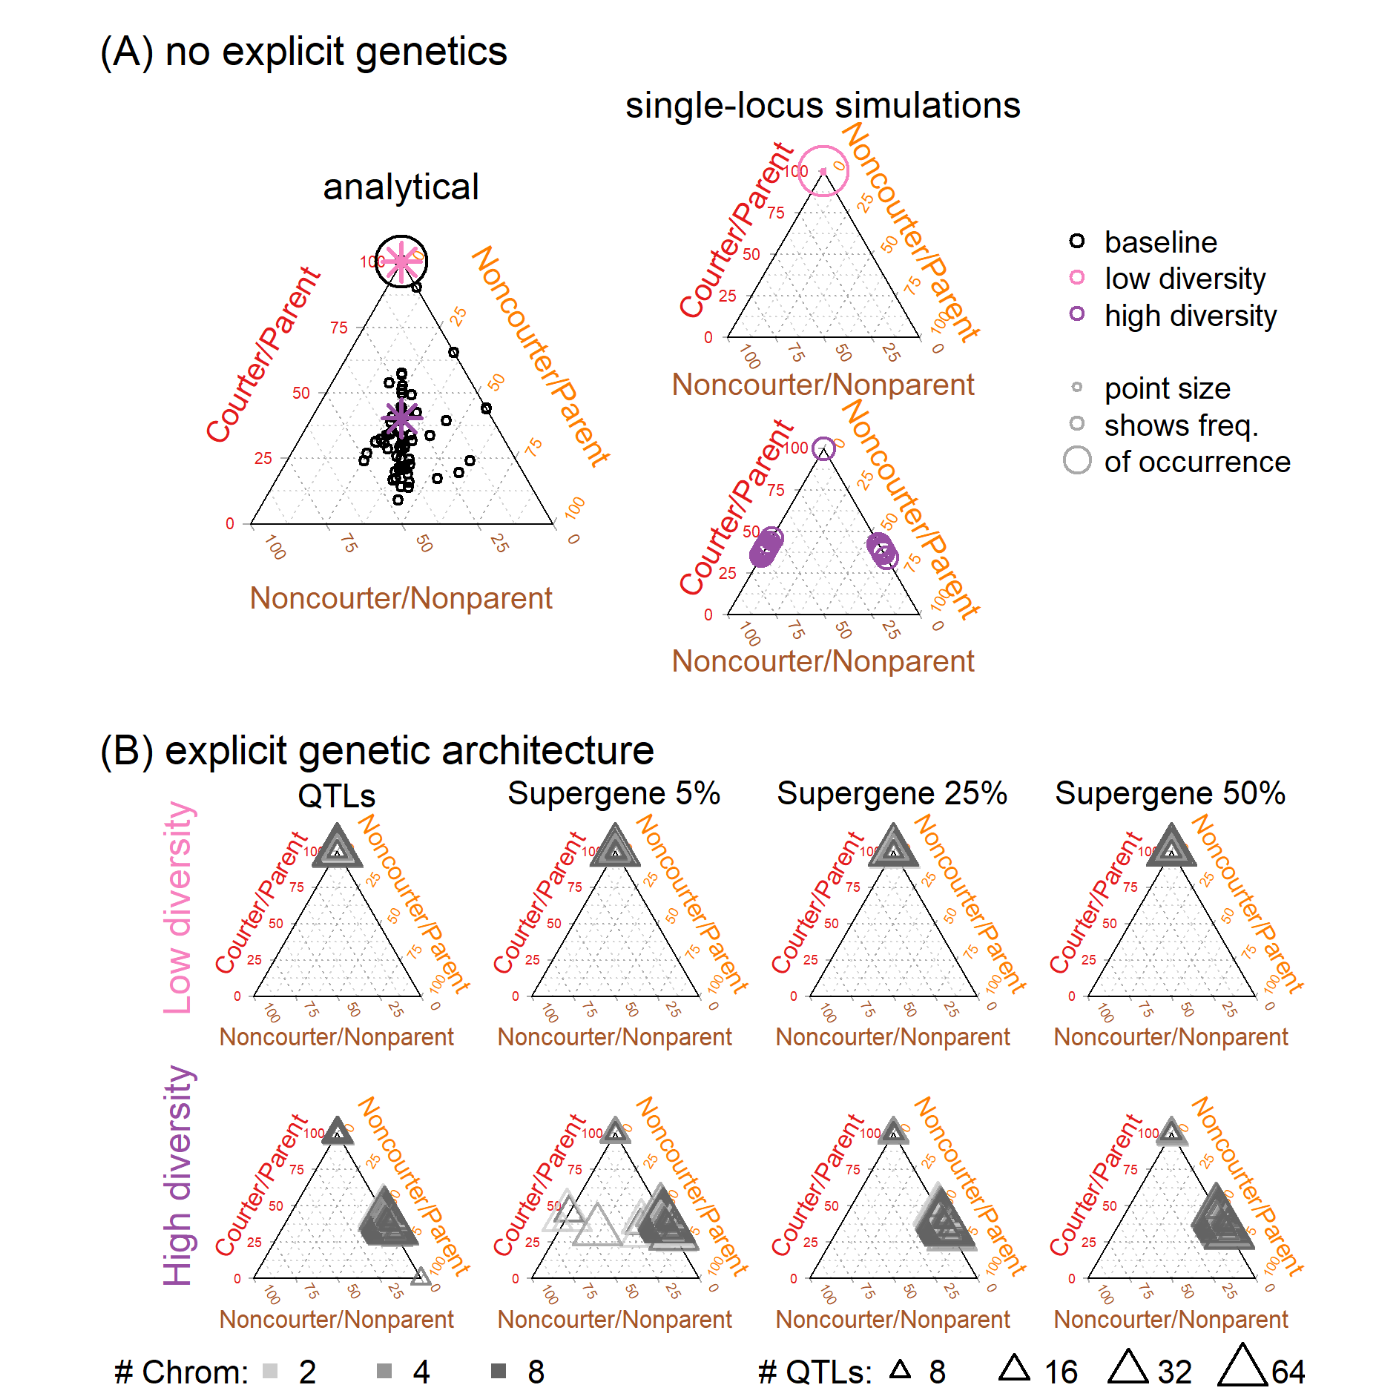
\includegraphics[width=0.9\linewidth,]{../figs/combinedTernaryTall-1} \caption{The inclusion of recombination and stochasticity alter
the frequency of male morphs and explicit genetic architectures affects
which morphs are maintained under balancing selection. In all diagrams,
each point in the triangle represents a different combination of the
predicted frequency of the three male morphs, where the corners
represent 100\% of each morph and each edge represents relative
percentages of two out of the three morphs. (A) A comparison of the
baseline analytical model and the architecture-free single-locus
simulations. In these diagrams, point size reflects the number of
parameter settings resulting in that exact combination of morph
frequencies. The left panel represents the predictions of the baseline
model, in which most parameter combinations result in the fixation of
the courter/parent morph but many retain three morphs. The outcomes of
the chosen low diversity and high diversity parameter sets are marked
with a purple and a pink asterisk, respectively. On the right are the
outputs from the individual-based simulation models without explicit
genetic architectures for the chosen low diversity parameters (top) and
high diversity parameters (bottom). Most low diversity replicates result
in fixation of the courter/parent, with some having one or two
non-courter/parent individuals in the final population, while the high
diversity replicates include maintenance of two morphs (courter/parent
and non-courter/parent or courter/parent and non-courter/non-parent) and
the fixation of the courter/parent morph. (B) Adding explicit genetic
architectures affects which morphs are maintained for the high diversity
parameters, but the number of QTLs or chromosomes are not driving
factors, and low diversity parameter settings resulted in the predicted
outcomes. The ternary diagrams show the final frequencies of the morphs
from individual-based simulations with QTLs distributed throughout the
genome (left column) or clustered into supergenes that make up 5\%, 25\%,
or 50\% of the chromosome the supergene is situated on. Colours represent
the number of chromosomes considered by the model and the size of the
points depict the number of QTLs underlying each trait. In low diversity
scenarios, regardless of genetic architecture, the courter-parent morph
is the one that is retained, same as in the baseline model and
architecture-free simulations in (A). Unlike in the baseline and
architecture-free models, in high diversity scenarios the
non-courter/non-parent individuals are rarely retained, and are only
retained in a few cases when supergenes are very tightly linked.}\label{fig:ternaryPlots}
\end{figure}

Overall, the parameters affecting whether diversity was maintained after
both 100 and 1000 generations were the initial frequencies of the
morphs, sperm competition (\(c\)), relative reproductive allocation (\(r\)),
and the number of sneakers allowed (\(n_{sneak}\)). Some initial starting
conditions took more than 100 generations to reach a consistent (i.e.,
equilibrial) state, but the contributions of the initial frequencies and
these three parameters remained qualitatively consistent between 100 and
1000 generations.

As expected, larger sperm competition coefficients (\(c\)) resulted in a
higher likelihood of non-courters being retained in the population,
which makes sense given that \(c\) affects the proportion of eggs within a
clutch that a non-courting male can successfully fertilize. Sperm
competition interacted with the reproductive allocation ratio, \(r\), such
that when \(c>0.2\), the maximum diversity was achieved when
\(0.5 \le r \le 1\). As an illustrative example, if \(r = 0.5\), \(c=0.2\),
and the non-courting male's number of eggs he can fertilize is 8, the
non-courting male would fertilize
\(\frac{(8)(2)}{(8) ( 0.5)+(2 )( 0.2 )( 8)}\) =
0.222 of the offspring. The effects of
sperm competition on morph diversity were further influenced by
\(n_{sneak}\), with larger contributions from an individual non-courting
male (e.g., larger \(c\)) being required to maintain diversity of morphs
when fewer sneakers were allowed (Fig. S1). This result makes sense
because the number of sneakers is multiplied by the sperm competition
coefficient to determine the proportion of offspring fertilized by the
non-courters for a given clutch. These analyses therefore helped to
build an understanding of how the different parameters affected model
predictions and provided a baseline against which to compare our
simulation results.

We used these results of the baseline model to select parameter values
for the individual-based simulation model. We selected one set of
parameters predicted to produce low-diversity populations (i.e., those
where only one morph were retained) and another set expected to produce
high-diversity populations (i.e., where 2 or more morphs were retained).
The chosen parameter values are shown in Table
\ref{tab:SimParamsTable}.

\begin{table}[H]

\caption{\label{tab:SimParamsTable}Table of parameters selected to create a high-diversity population. All morphs started at equal frequencies.}
\centering
\begin{tabular}[t]{lrr}
\toprule
Parameter & Low Diversity Value & High Diversity Value\\
\midrule
Ratio of reproductive investment, r (courter to non-courter ratio) & 2.0 & 0.70\\
Max number of offspring CP males can produce & 8.0 & 6.00\\
Max number of offspring CN males can produce & 8.0 & 6.00\\
Max number of offspring NP males can produce & 4.0 & 8.00\\
Max number of offspring NN males can produce & 4.0 & 8.00\\
\addlinespace
c (sperm competition coefficient) & 0.5 & 0.75\\
number of sneakers & 2.0 & 2.00\\
\bottomrule
\end{tabular}
\end{table}

\hypertarget{recombination-mutation-and-stochasticity-result-in-fewer-morphs-maintained}{%
\subsection{Recombination, mutation, and stochasticity result in fewer morphs maintained}\label{recombination-mutation-and-stochasticity-result-in-fewer-morphs-maintained}}

A striking difference between the analytical model and the simple
Mendelian simulation model is that only two morphs are maintained with
parameters that retained three morphs in the analytical model (Fig.
\ref{fig:ternaryPlots}A; see Fig. S2 for outcomes with alternative
mating dynamics). Furthermore, stochasticity played a major role in
which morph co-existed with the courter/parent morph, even when the
parameter values used were identical (Fig. S3). Variation in outcomes
among replicate runs can be attributed to the many sources of random
chance incorporated in the model: stochasticity associated with finite
population sizes (i.e., genetic drift), the randomness of recombination,
and the finite mate search process (in which females might not find a
suitable mate, even if one exists in the population) all contribute to
the within-replicate variation observed. Altogether, including realistic
genetic components reduced the total diversity of morphs compared to a
deterministic single-gene model.

\hypertarget{polygenic-architectures-reduce-effects-of-stochasticity-with-supergenes-having-little-effect-on-the-maintenance-of-morphs}{%
\subsubsection{Polygenic architectures reduce effects of stochasticity, with supergenes having little effect on the maintenance of morphs}\label{polygenic-architectures-reduce-effects-of-stochasticity-with-supergenes-having-little-effect-on-the-maintenance-of-morphs}}

In the low diversity parameter space, the outcomes remained consistent
with the single-locus model (and the predictions of the mathematical
model): courter/parents dominated the populations, with complete
fixation of the morph in the majority of runs, and any variation
existing in the form of 1-2 individuals (courter/parent frequencies were
\(\ge\) 99\% in all cases), which were a result of stochasticity and
recombination as opposed to balancing selection favouring multiple
morphs (Fig. S4). These results were consistent across all genetic
architectures, including QTLs distributed across 2, 4, and 8 chromosomes
and QTLs clustered in supergenes spanning from 5\% to 50\% of a single
chromosome. In the high diversity parameter space, polygenic loci
distributed throughout the genome resulted in the maintenance of the
courter/parent trait at a frequency of
50.7\%
(\(\pm\)
1.59\%),
with the non-courter/parent being the dominant morph. These proportions
are remarkably consistent across genetic architectures (Fig.
\ref{fig:ternaryPlots}B). Most simulations with supergenes resulted in
very similar final morph frequencies
(49.21\%
\(\pm\)
0.88\%),
and only occasionally resulted in either three morphs being retained or
the non-courter/non-parent morph replacing the non-courter/parent. The
size of the supergene did not substantially affect the final morph
frequencies, nor did the total number of QTLs underlying each locus. A
consequence of the stabilisation of morph frequencies was a reduction in
the strength of selection acting in the final generation relative to the
first generation of the model (Fig. S5).

Our initial expectation was that supergenes would follow a pattern more
similar to the single locus results, because empirical examples have
demonstrated Mendelian inheritance patterns approximating single-locus
models (e.g., {[}19{]}).
To better understand the reasons for the similarity between the the
genome-wide QTLs simulations versus the supergene simulations, we
visualised the QTL haplotypes in supergenes (see Fig. S6 and S7 for
representative images). These visualisations suggest that because of the
additive, polygenic nature of our traits, individuals have multiple
pathways to creating the morphs in terms of genotypes at each QTL, even
when QTLs are segregating together in a supergene. These findings
suggest that supergenes are not necessary for maintaining multiple
reproductive morphs that are comprised of many causal loci.

\hypertarget{genome-wide-genetic-diversity-is-maintained-even-when-trait-diversity-is-low}{%
\subsubsection{Genome-wide genetic diversity is maintained even when trait diversity is low}\label{genome-wide-genetic-diversity-is-maintained-even-when-trait-diversity-is-low}}

Supergenes enable specific combinations of alleles at multiple loci to
be inherited together as a single haplotype; as such, we expected that
the simulations with supergenes would evolve to have lower within-morph
genetic diversity at QTLs (i.e., low observed heterozygosity) than the
genome-wide QTLs scenarios. Surprisingly, we found that the average
genome-wide expected heterozygosity was not substantially different in
simulations with genome-wide QTLs versus QTLs in supergenes in the final
generation of the simulations (t = -0.31, df = 326.75, p = -0.31;
genome-wide mean = 0.15, supergene mean = 0.16; Fig.
\ref{fig:genomewideDiv} A; Fig. S8). In most runs, the heterozygosity
at QTLs was did not significantly differ from heterozygosity at neutral
markers (mean p-value from t-tests is 0.5 ± 0.01). Tajima's D, which
tests for directional or balancing selection, also reflects genetic
variation in a sequence of DNA, and did not deviate substantially
between genetic architectures and did not relate to final morph
frequencies (Fig. \ref{fig:genomewideDiv} B; Fig. S8). Average linkage
disequilibrium was higher for QTLs in supergenes than
randomly-distributed QTLs (Fig. S9).

Similarly, we expected supergenes to show more differentiation between
morphs, since their QTLs segregated together. However, \(G_{ST}\) between
male morphs was also not predicted by the frequency of courter/parent
morphs (Fig. \ref{fig:genomewideDiv} C; Fig. S9). Significant peaks in
genome-wide \(G_{ST}\) estimates were identified, and we evaluated whether
QTLs were located near to those \(G_{ST}\) peaks (i.e., we identified if
\(G_{ST}\) outliers were associated with true QTLs). From this, we then
calculated the proportion of true QTLs that were located in these
significant \(G_{ST}\) peaks, and found that under high-diversity
parameters, on average 63.04
\(\pm\) 1.09\%, of randomly
distributed QTLs and and
74.31 \(\pm\)
0.9\% of QTLs in supergenes
were found in \(G_{ST}\) peaks, irrespective of the courter/parent
frequency (Fig. S10).

\begin{figure}[H]
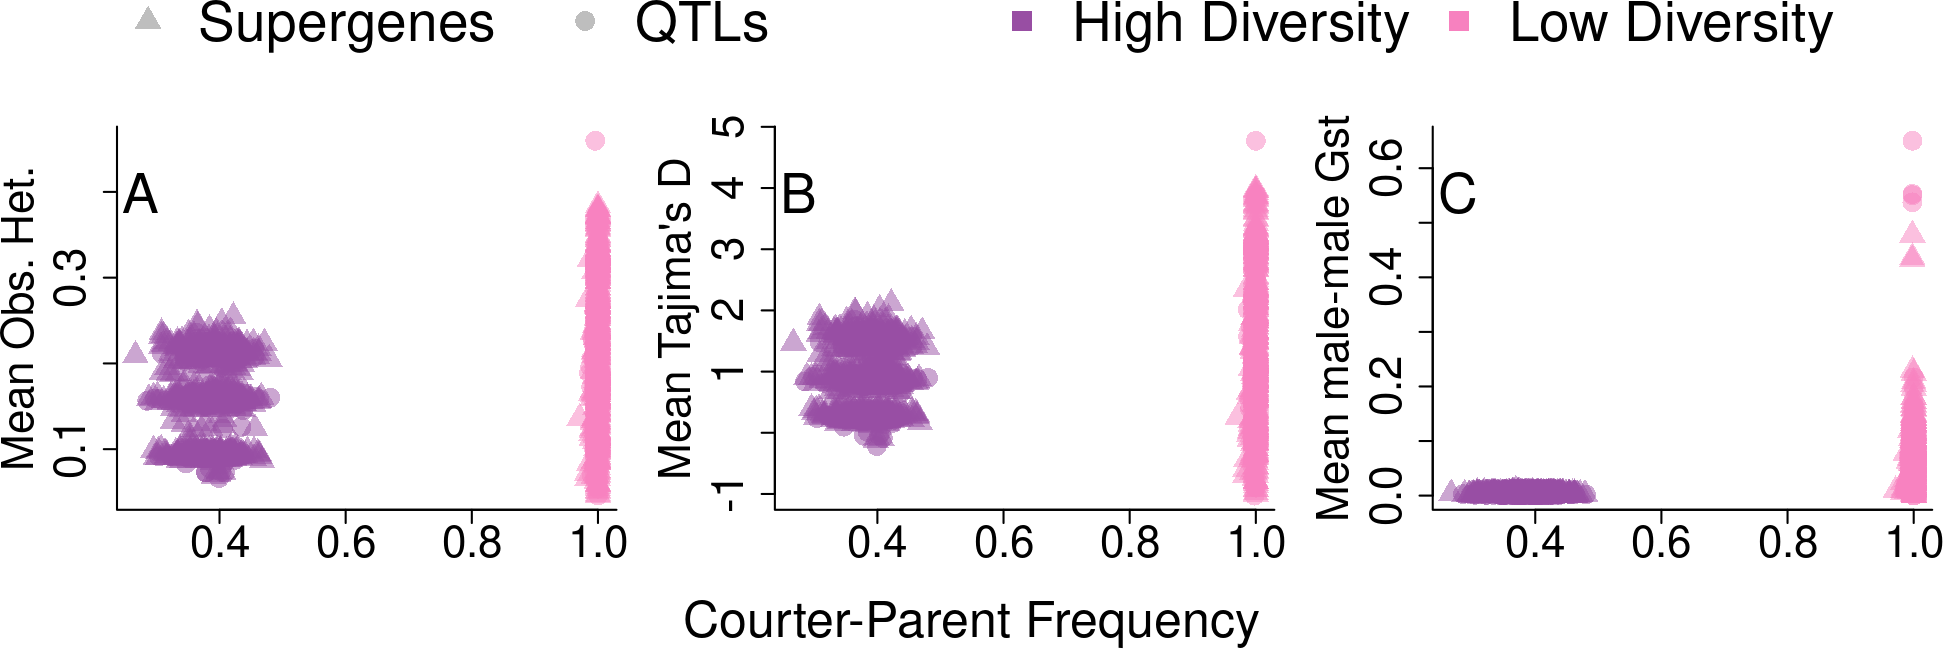
\includegraphics[width=9.71in,]{../figs/genomewideDiv-1} \caption{Genome-wide genetic diversity in the final generation of the simulations was not influcenced by genetic architecture or the phenotypic diversity (i.e., morph frequencies), but did differ between low- and high-diversity parameter settings. Shown are genome-wide observed heterozygosity (A), Tajima’s D (B), and male-male Gst (C).}\label{fig:genomewideDiv}
\end{figure}

A consequence of this high genetic diversity underpinning the
categorical traits appears to be high error rates in detecting true QTLs
using genome-wide association tests. As expected, the detection of true
QTLs in a GWAS was more likely when fewer QTLs underpin the trait,
especially if those QTLs are aggregated on fewer chromosomes (Fig. S11).
The type of genetic architecture (genome-wide QTLs versus supergenes)
had a minimal effect on the detection of QTLs. The QTLs for parent
traits were more reliably detected by GWAS than the courter QTLs, even
though in the majority of simulations the final population only
contained parental males (Fig. \ref{fig:ternaryPlots}B). The higher
probability of detecting parent QTLs could be attributed to stronger
selection on that trait (i.e., being a non-parent was more costly than
being a non-courter). To summarise, a surprising degree of genetic
diversity was retained in our simulations despite fixation of some
morphs, which impeded the detection of causal loci.

\hypertarget{discussion}{%
\section{Discussion}\label{discussion}}

Understanding how the genetic architecture of phenotypic polymorphisms
facilitates or constrains their maintenance and evolution is crucial for
understanding the mechanisms shaping diversity. Yet, we do not fully
understand how polygenic phenotypes can be inherited as discrete suites
of traits. Using a simulation model, we show that the genetic
architecture -- specifically, the number of loci and the extent of
linkage among them -- affects the persistence of complex discrete
phenotypes. In our single-gene models, under parameter conditions that
favoured the maintenance of multiple morphs in simple single-gene
models, which male morphs were retained was determined due to
stochasticity. However, when more complex architectures are modelled
using the same parameters, specific combinations of morphs were
retained; thus, genetic complexity of traits reduced the importance of
stochasticity. This phenomenon was likely due to genetic correlations
between traits and loci. In contrast to expectations, we did not find
that supergenes increased the probability that multiple morphs are
maintained in the population. QTLs organised into supergenes (in which
causal SNPs are physically co-located and experience reduced
recombination), although associated with high linkage disequilibrium,
did not have qualitatively different outcomes in terms of the
maintenance of discrete morphs than QTLs distributed genome-wide. In
addition, unexpectedly high levels of genetic diversity were retained
within morphs in the supergene scenarios.

\hypertarget{supergenes-have-similar-outcomes-to-randomly-distributed-qtls}{%
\subsection{Supergenes have similar outcomes to randomly distributed QTLs}\label{supergenes-have-similar-outcomes-to-randomly-distributed-qtls}}

The discovery of supergenes underlying polymorphism was hailed as an
explanation for how complex suites of traits could be inherited in a
discrete manner, when they must also be polygenic
{[}55{]}. We provide compelling
evidence that additive genetic variation need not be co-located in a
non-recombining region of a chromosome for multiple morphs to be
maintained. Our model makes several assumptions that might differ from
real-world examples, however, and These additional forms of complexity
in genetic architectures are fruitful areas for future research. For
example, the steroid hormone receptor genes in white-throated sparrow
and ruff supergenes {[}26{]} would be better
approximated by a logarithmic distribution, which differs from the
additive distribution of allelic effects that we used. Additionally,
many polymorphisms could rely on dominance hierarchies (e.g., as
modelled by {[}10{]}), and could even
be underpinned by dominance reversals between morphs
{[}25{]} or sexes
{[}56{]}, which were not
possibilities considered in our model. Regardless, we provide the
important result that discrete morphs can be maintained within
populations even without discrete genetic architectures with a
threshold-based switch, contrary to predictions from some authors
{[}57{]}. Our results indicate that
discrete morphs need not have causal genes co-located in a supergene but
can still follow the single- or two-locus phenotypic inheritance
patterns seen in side-blotched lizards {[}7{]}
and damselflies {[}10{]}.

\hypertarget{unexpected-genetic-variation-was-maintained-even-when-traits-were-fixed}{%
\subsection{Unexpected genetic variation was maintained even when traits were fixed}\label{unexpected-genetic-variation-was-maintained-even-when-traits-were-fixed}}

Comparing our model predictions to predictions from the literature on
sexually antagonistic selection on autosomes can be informative because
both scenarios involve balancing selection on shared genomic regions
{[}13{]}. In our model, balancing
selection arises from fitness tradeoffs between reproductive investment
and survival in males, which creates conflicts among morphs, wheeras
autosomal sexually antagonistic selection involves conflicts between
sexes over similar tradeoffs. Unlike models of sex-specific selection,
which have found that under conditions resulting in balancing selection
on males and females genetic variation can be maintained
{[}58{]}, but that most genomic regions
will not show excessive variation
{[}40{]}, our models predict the
maintenance of variation in phenotypes and in genotypes. Additionally,
we detected high levels of genetic differentiation between male types,
even without strong selection, which is opposite to the predictions for
sex-specific selection {[}59{]}. As such,
our model highlights how demographic factors, stochasticity, and genomic
effects such as pleiotropy and linkage can affect genetic variation, and
potentially obscure putative genome-wide signals of selection.

Furthermore, we expected the supergenes to evolve to contain single
haplotypes for each morph, as has been reported in empirical examples of
supergenes controlling complex phenotypes (e.g.,
{[}19{]};
{[}20{]};
{[}22{]};
{[}5{]}). A striking difference in
our results from those of the empirical examples is that we do not see
fixed alleles exclusively in one morph or the other. Instead,
quantitative variation is retained within the supergenes, and we do not
observe discrete haplotypes underlying the categorical morphs. If we
compare our supergene results to our QTL results, as expected, linkage
disequilibrium was elevated within the supergene region in our model,
and similarly high levels of LD were not observed in the genome-wide QTL
models (Fig. S10). However, measures of genetic variation and
between-morph differentiation were similar in the two types of models
(Fig. \ref{fig:genomewideDiv}).

These unexpected levels of genetic diversity might have also impaired
our ability to detect the causal QTLs using methods such as genome-wide
association studies. We only identified \(\le\) 50\% of true QTLs, with
many false positives. Low true positives and high false positives are
consistent with other simulation studies of genome-wide studies of
selection and trait associations
{[}40{]}, especially for genome-wide
associations with dichotomous traits
{[}35{]}. In this study, these
limitations are consistent with both genetic architectures, so appears
to not only be driven by the extreme linkage disequilibrium within
supergenes that makes associations difficult to identify
{[}22{]}. Our results suggest that
genome-wide association studies alone are likely to miss key causal
variants, even if such approaches have been sufficient in identifying
causal regions in some species
{[}5,16,19,20,22,24{]}.

\hypertarget{summary}{%
\subsection{Summary}\label{summary}}

Here, we show that the genetic architecture of discrete morphs affects
the frequency of morphs maintained under balancing selection, but does
not fundamentally change the conditions enabling balancing selection to
allow multiple morphs to persist. We also show surprisingly elevated
genetic diversity can be maintained, but that genome-wide scans are
unlikely to accurately identify the complete genetic architecture of
discrete traits. Our results highlight that additively determined
dichotomous traits can be polygenic and exhibit evolutionary dynamics
equivalent to a single-locus model, regardless of the physical
configuration of the causal variants.

\hypertarget{acknowledgments}{%
\section{Acknowledgments}\label{acknowledgments}}

Thanks to the Flanagan lab for their feedback on early drafts of this
work. We acknowledge Ngāi Tūāhuriri, upon whose lands the analyses and
writing was conducted. This work was conducted in part while SPF was a
postdoctoral fellow at the National Institute for Mathematical and
Biological Synthesis, sponsored by the National Science Foundation
through NSF Award \#DBI-1300426, with additional support from The
University of Tennessee, Knoxville. SPF was partially funded by the
Marsden fund grant number UOC1904 while working on this research. SHA
acknowledges support from funding from the National Science Foundation
(Grants IOS-1522491 and IOS-1655297) and the University of California
Santa Cruz.

\hypertarget{data-accessibility}{%
\section{Data Accessibility}\label{data-accessibility}}

All code is maintained on github (\url{https://github.com/spflanagan/ARTs})
and the current version has been archived on Zenodo (DOI: ). Outputs
used in the creation of figures in the main text and the supplement are
archived on zenodo (DOI: 10.5281/zenodo.8248198).

\hypertarget{author-contributions}{%
\section{Author Contributions}\label{author-contributions}}

SPF and SHA conceived of the project. SPF wrote code and performed
analysis with input from SHA. SPF wrote the first draft of the
manuscript and both authors substantially revised subsequent version.
Both authors approve the the submitted version of the manuscript.

\hypertarget{references}{%
\section*{References}\label{references}}
\addcontentsline{toc}{section}{References}

\hypertarget{refs}{}
\begin{CSLReferences}{0}{0}
\leavevmode\vadjust pre{\hypertarget{ref-oliveiraAlternativeReproductiveTactics2008}{}}%
\CSLLeftMargin{1. }%
\CSLRightInline{Oliveira RF, Taborsky M, Brockmann HJ. 2008 \emph{Alternative {Reproductive Tactics}: {An Integrative Approach}}. {Cambridge, United Kingdom}: {Cambridge University Press}. }

\leavevmode\vadjust pre{\hypertarget{ref-iserbytNegativeFrequencydependentSelection2013}{}}%
\CSLLeftMargin{2. }%
\CSLRightInline{Iserbyt A, Bots J, Van Gossum H, Sherratt TN. 2013 Negative frequency-dependent selection or alternative reproductive tactics: Maintenance of female polymorphism in natural populations. \emph{BMC Evolutionary Biology} \textbf{13}, 139. (doi:\href{https://doi.org/10.1186/1471-2148-13-139}{10.1186/1471-2148-13-139})}

\leavevmode\vadjust pre{\hypertarget{ref-prykeFrequencydependentPhysiologicalTradeoffs2007}{}}%
\CSLLeftMargin{3. }%
\CSLRightInline{Pryke SR, Astheimer LB, Buttemer WA, Griffith SC. 2007 Frequency-dependent physiological trade-offs between competing colour morphs. \emph{Biology Letters} \textbf{3}, 494--497. (doi:\href{https://doi.org/10.1098/rsbl.2007.0213}{10.1098/rsbl.2007.0213})}

\leavevmode\vadjust pre{\hypertarget{ref-alonzoMateChoiceGames2001}{}}%
\CSLLeftMargin{4. }%
\CSLRightInline{Alonzo SH, Sinervo B. 2001 Mate choice games, context-dependent good genes, and genetic cycles in the side-blotched lizard, {\emph{Uta}}{ \emph{Stansburiana}}. \emph{Behavioral Ecology and Sociobiology} \textbf{49}, 176--186. (doi:\href{https://doi.org/10.1007/s002650000265}{10.1007/s002650000265})}

\leavevmode\vadjust pre{\hypertarget{ref-hendrickxMasculinizingSupergeneUnderlies2022}{}}%
\CSLLeftMargin{5. }%
\CSLRightInline{Hendrickx F, De Corte Z, Sonet G, Van Belleghem SM, Köstlbacher S, Vangestel C. 2022 A masculinizing supergene underlies an exaggerated male reproductive morph in a spider. \emph{Nature Ecology \& Evolution} \textbf{6}, 195--206. (doi:\href{https://doi.org/10.1038/s41559-021-01626-6}{10.1038/s41559-021-01626-6})}

\leavevmode\vadjust pre{\hypertarget{ref-mankSexspecificMorphsGenetics2022}{}}%
\CSLLeftMargin{6. }%
\CSLRightInline{Mank JE. 2022 Sex-specific morphs: The genetics and evolution of intra-sexual variation. \emph{Nature Reviews Genetics}, 1--9. (doi:\href{https://doi.org/10.1038/s41576-022-00524-2}{10.1038/s41576-022-00524-2})}

\leavevmode\vadjust pre{\hypertarget{ref-sinervoRunawaySocialGames2001}{}}%
\CSLLeftMargin{7. }%
\CSLRightInline{Sinervo B. 2001 Runaway social games, genetic cycles driven by alternative male and female strategies, and the origin of morphs. \emph{Genetica} \textbf{112--113}, 417--434. (doi:\href{https://doi.org/10.1007/978-94-010-0585-2_25}{10.1007/978-94-010-0585-2\_25})}

\leavevmode\vadjust pre{\hypertarget{ref-sinervoRockPaperScissors1996}{}}%
\CSLLeftMargin{8. }%
\CSLRightInline{Sinervo B, Lively CM. 1996 The rock\textendash paper\textendash scissors game and the evolution of alternative male strategies. \emph{Nature} \textbf{380}, 240--243. (doi:\href{https://doi.org/10.1038/380240a0}{10.1038/380240a0})}

\leavevmode\vadjust pre{\hypertarget{ref-takahashiNegativeFrequencydependentSelection2010}{}}%
\CSLLeftMargin{9. }%
\CSLRightInline{Takahashi Y, Yoshimura J, Morita S, Watanabe M. 2010 Negative frequency-dependent selection in female color polymorphism of a damselfly. \emph{Evolution} \textbf{64}, 3620--3628. (doi:\href{https://doi.org/10.1111/j.1558-5646.2010.01083.x}{10.1111/j.1558-5646.2010.01083.x})}

\leavevmode\vadjust pre{\hypertarget{ref-svenssonFemalePolymorphismFrequency2005}{}}%
\CSLLeftMargin{10. }%
\CSLRightInline{Svensson EI, Abbott J, Härdling R. 2005 Female polymorphism, frequency dependence, and rapid evolutionary dynamics in natural populations. \emph{The American Naturalist} \textbf{165}, 567--576. (doi:\href{https://doi.org/10.1086/429278}{10.1086/429278})}

\leavevmode\vadjust pre{\hypertarget{ref-sinervoDevelopmentalPhysiologicalNeural2006}{}}%
\CSLLeftMargin{11. }%
\CSLRightInline{Sinervo B, Calsbeek R. 2006 \href{https://www.jstor.org/stable/30033844}{The developmental, physiological, neural, and genetical causes and consequences of frequency-dependent selection in the wild}. \emph{Annual Review of Ecology, Evolution, and Systematics} \textbf{37}, 581--610.}

\leavevmode\vadjust pre{\hypertarget{ref-ryanGeneticPolymorphismSwordtail1992}{}}%
\CSLLeftMargin{12. }%
\CSLRightInline{Ryan MJ, Pease CM, Morris MR. 1992 A genetic polymorphism in the swordtail {\emph{Xiphophorus}}{ \emph{Nigrensis}}: Testing the prediction of equal fitnesses. \emph{The American Naturalist} \textbf{139}, 21--31.}

\leavevmode\vadjust pre{\hypertarget{ref-morrisIntralocusTacticalConflict2013}{}}%
\CSLLeftMargin{13. }%
\CSLRightInline{Morris MR, Goedert D, Abbott JK, Robinson DM, Rios-Cardenas O. 2013 Intralocus {Tactical Conflict} and the {Evolution} of {Alternative Reproductive Tactics}. In \emph{Advances in the {Study} of {Behavior}}, pp. 447--478. {Elsevier}. (doi:\href{https://doi.org/10.1016/B978-0-12-407186-5.00007-0}{10.1016/B978-0-12-407186-5.00007-0})}

\leavevmode\vadjust pre{\hypertarget{ref-sinervoCorrelationalSelectionEvolution2002}{}}%
\CSLLeftMargin{14. }%
\CSLRightInline{Sinervo B, Svensson E. 2002 Correlational selection and the evolution of genomic architecture. \emph{Heredity} \textbf{89}, 329--338. (doi:\href{https://doi.org/10.1038/sj.hdy.6800148}{10.1038/sj.hdy.6800148})}

\leavevmode\vadjust pre{\hypertarget{ref-tsubakiGeneticPolymorphismLinked2003a}{}}%
\CSLLeftMargin{15. }%
\CSLRightInline{Tsubaki Y. 2003 The genetic polymorphism linked to mate-securing strategies in the male damselfly {\emph{Mnais}}{ \emph{Costalis}} {Selys} ({Odonata}: {Calopterygidae}). \emph{Population Ecology} \textbf{45}, 263--266. (doi:\href{https://doi.org/10.1007/s10144-003-0162-8}{10.1007/s10144-003-0162-8})}

\leavevmode\vadjust pre{\hypertarget{ref-kimGeneticsEvidenceBalancing2019}{}}%
\CSLLeftMargin{16. }%
\CSLRightInline{Kim K-W \emph{et al.} 2019 Genetics and evidence for balancing selection of a sex-linked colour polymorphism in a songbird. \emph{Nature Communications} \textbf{10}, 1--11. (doi:\href{https://doi.org/10.1038/s41467-019-09806-6}{10.1038/s41467-019-09806-6})}

\leavevmode\vadjust pre{\hypertarget{ref-slyMolecularParallelismSignaling2022}{}}%
\CSLLeftMargin{17. }%
\CSLRightInline{Sly ND, Freeman-Gallant CR, Henschen AE, Minias P, Whittingham LA, Dunn PO. 2022 Molecular parallelism in signaling function across different sexually selected ornaments in a warbler. \emph{Proceedings of the National Academy of Sciences} \textbf{119}, e2120482119. (doi:\href{https://doi.org/10.1073/pnas.2120482119}{10.1073/pnas.2120482119})}

\leavevmode\vadjust pre{\hypertarget{ref-flanaganGenomewideSelectionComponents2017}{}}%
\CSLLeftMargin{18. }%
\CSLRightInline{Flanagan SP, Jones AG. 2017 Genome-wide selection components analysis in a fish with male pregnancy. \emph{Evolution} \textbf{71}, 1096--1105. (doi:\href{https://doi.org/10.1111/evo.13173}{10.1111/evo.13173})}

\leavevmode\vadjust pre{\hypertarget{ref-lamichhaneyStructuralGenomicChanges2016}{}}%
\CSLLeftMargin{19. }%
\CSLRightInline{Lamichhaney S \emph{et al.} 2016 Structural genomic changes underlie alternative reproductive strategies in the ruff ({Philomachus} pugnax). \emph{Nat Genet} \textbf{48}, 84--88. (doi:\href{10.1038/ng.3430\%20http://www.nature.com/ng/journal/v48/n1/abs/ng.3430.html\#supplementary-information}{10.1038/ng.3430 http://www.nature.com/ng/journal/v48/n1/abs/ng.3430.html\#supplementary-information})}

\leavevmode\vadjust pre{\hypertarget{ref-kupperSupergeneDeterminesHighly2016}{}}%
\CSLLeftMargin{20. }%
\CSLRightInline{Kupper C \emph{et al.} 2016 A supergene determines highly divergent male reproductive morphs in the ruff. \emph{Nat Genet} \textbf{48}, 79--83. (doi:\href{10.1038/ng.3443\%20http://www.nature.com/ng/journal/v48/n1/abs/ng.3443.html\#supplementary-information}{10.1038/ng.3443 http://www.nature.com/ng/journal/v48/n1/abs/ng.3443.html\#supplementary-information})}

\leavevmode\vadjust pre{\hypertarget{ref-thomasChromosomalPolymorphismLinked2008}{}}%
\CSLLeftMargin{21. }%
\CSLRightInline{Thomas JW, Cáceres M, Lowman JJ, Morehouse CB, Short ME, Baldwin EL, Maney DL, Martin CL. 2008 The chromosomal polymorphism linked to variation in social behavior in the white-throated sparrow ({\emph{Zonotrichia Albicollis}}) is a complex rearrangement and suppressor of recombination. \emph{Genetics} \textbf{179}, 1455--1468. (doi:\href{https://doi.org/10.1534/genetics.108.088229}{10.1534/genetics.108.088229})}

\leavevmode\vadjust pre{\hypertarget{ref-kimSexlinkedSupergeneControls2017}{}}%
\CSLLeftMargin{22. }%
\CSLRightInline{Kim K-W, Bennison C, Hemmings N, Brookes L, Hurley LL, Griffith SC, Burke T, Birkhead TR, Slate J. 2017 A sex-linked supergene controls sperm morphology and swimming speed in a songbird. \emph{Nature Ecology \& Evolution} \textbf{1}, 1168--1176. (doi:\href{https://doi.org/10.1038/s41559-017-0235-2}{10.1038/s41559-017-0235-2})}

\leavevmode\vadjust pre{\hypertarget{ref-kniefSexchromosomeInversionCauses2017}{}}%
\CSLLeftMargin{23. }%
\CSLRightInline{Knief U \emph{et al.} 2017 A sex-chromosome inversion causes strong overdominance for sperm traits that affect siring success. \emph{Nature Ecology \& Evolution} \textbf{1}, 1177--1184. (doi:\href{https://doi.org/10.1038/s41559-017-0236-1}{10.1038/s41559-017-0236-1})}

\leavevmode\vadjust pre{\hypertarget{ref-gazdaGeneticMechanismSexual2020}{}}%
\CSLLeftMargin{24. }%
\CSLRightInline{Gazda MA \emph{et al.} 2020 A genetic mechanism for sexual dichromatism in birds. \emph{Science} \textbf{368}, 1270--1274.}

\leavevmode\vadjust pre{\hypertarget{ref-pearseSexdependentDominanceMaintains2019}{}}%
\CSLLeftMargin{25. }%
\CSLRightInline{Pearse DE \emph{et al.} 2019 Sex-dependent dominance maintains migration supergene in rainbow trout. \emph{Nature Ecology \& Evolution} \textbf{3}, 1731--1742. (doi:\href{https://doi.org/10.1038/s41559-019-1044-6}{10.1038/s41559-019-1044-6})}

\leavevmode\vadjust pre{\hypertarget{ref-maneySupergenesSteroids2022}{}}%
\CSLLeftMargin{26. }%
\CSLRightInline{Maney DL, Küpper C. 2022 Supergenes on steroids. \emph{Philosophical Transactions of the Royal Society B: Biological Sciences} \textbf{377}, 20200507. (doi:\href{https://doi.org/10.1098/rstb.2020.0507}{10.1098/rstb.2020.0507})}

\leavevmode\vadjust pre{\hypertarget{ref-merrittSupergenelinkedEstrogenReceptor2020}{}}%
\CSLLeftMargin{27. }%
\CSLRightInline{Merritt JR, Grogan KE, Zinzow-Kramer WM, Sun D, Ortlund EA, Yi SV, Maney DL. 2020 A supergene-linked estrogen receptor drives alternative phenotypes in a polymorphic songbird. \emph{Proceedings of the National Academy of Sciences} \textbf{117}, 21673--21680. (doi:\href{https://doi.org/10.1073/pnas.2011347117}{10.1073/pnas.2011347117})}

\leavevmode\vadjust pre{\hypertarget{ref-maneySupergeneBirdFour2020}{}}%
\CSLLeftMargin{28. }%
\CSLRightInline{Maney DL, Merritt JR, Prichard MR, Horton BM, Yi SV. 2020 Inside the supergene of the bird with four sexes. \emph{Hormones and Behavior} \textbf{126}, 104850. (doi:\href{https://doi.org/10.1016/j.yhbeh.2020.104850}{10.1016/j.yhbeh.2020.104850})}

\leavevmode\vadjust pre{\hypertarget{ref-lepaisGeneticArchitectureThreshold2017}{}}%
\CSLLeftMargin{29. }%
\CSLRightInline{Lepais O, Manicki A, Glise S, Buoro M, Bardonnet A. 2017 Genetic architecture of threshold reaction norms for male alternative reproductive tactics in {Atlantic} salmon ({Salmo} salar {L}.). \emph{Scientific Reports} \textbf{7}, 43552. (doi:\href{https://doi.org/10.1038/srep43552}{10.1038/srep43552})}

\leavevmode\vadjust pre{\hypertarget{ref-nugentNeuroendocrineProfilesAssociated2016}{}}%
\CSLLeftMargin{30. }%
\CSLRightInline{Nugent BM, Stiver KA, Alonzo SH, Hofmann HA. 2016 Neuroendocrine profiles associated with discrete behavioural variation in {Symphodus} ocellatus, a species with male alternative reproductive tactics. \emph{Molecular Ecology} \textbf{25}, 5212--5227. (doi:\href{https://doi.org/10.1111/mec.13828}{10.1111/mec.13828})}

\leavevmode\vadjust pre{\hypertarget{ref-stuglikAlternativeReproductiveTactics2014}{}}%
\CSLLeftMargin{31. }%
\CSLRightInline{Stuglik MT, Babik W, Prokop Z, Radwan J. 2014 Alternative reproductive tactics and sex-biased gene expression: The study of the bulb mite transcriptome. \emph{Ecology and Evolution} \textbf{4}, 623--632. (doi:\href{https://doi.org/10.1002/ece3.965}{10.1002/ece3.965})}

\leavevmode\vadjust pre{\hypertarget{ref-takahashiCandidateGenesAssociated2019}{}}%
\CSLLeftMargin{32. }%
\CSLRightInline{Takahashi M, Takahashi Y, Kawata M. 2019 Candidate genes associated with color morphs of female-limited polymorphisms of the damselfly {\emph{Ischnura}}{ \emph{Senegalensis}}. \emph{Heredity} \textbf{122}, 81--92. (doi:\href{https://doi.org/10.1038/s41437-018-0076-z}{10.1038/s41437-018-0076-z})}

\leavevmode\vadjust pre{\hypertarget{ref-josephsWhatCanGenomewide2017}{}}%
\CSLLeftMargin{33. }%
\CSLRightInline{Josephs EB, Stinchcombe JR, Wright SI. 2017 What can genome-wide association studies tell us about the evolutionary forces maintaining genetic variation for quantitative traits? \emph{New Phytologist} \textbf{214}, 21--33. (doi:\href{https://doi.org/10.1111/nph.14410}{10.1111/nph.14410})}

\leavevmode\vadjust pre{\hypertarget{ref-uricchioEvolutionaryPerspectivesPolygenic2020}{}}%
\CSLLeftMargin{34. }%
\CSLRightInline{Uricchio LH. 2020 Evolutionary perspectives on polygenic selection, missing heritability, and {GWAS}. \emph{Human Genetics} \textbf{139}, 5--21. (doi:\href{https://doi.org/10.1007/s00439-019-02040-6}{10.1007/s00439-019-02040-6})}

\leavevmode\vadjust pre{\hypertarget{ref-stringerUnderestimatedEffectSizes2011}{}}%
\CSLLeftMargin{35. }%
\CSLRightInline{Stringer S, Wray NR, Kahn RS, Derks EM. 2011 Underestimated effect sizes in {GWAS}: Fundamental limitations of single {SNP} analysis for dichotomous phenotypes. \emph{PLOS ONE} \textbf{6}, e27964. (doi:\href{https://doi.org/10.1371/journal.pone.0027964}{10.1371/journal.pone.0027964})}

\leavevmode\vadjust pre{\hypertarget{ref-bitarelloInferringBalancingSelection2023}{}}%
\CSLLeftMargin{36. }%
\CSLRightInline{Bitarello BD, Brandt DYC, Meyer D, Andrés AM. 2023 Inferring balancing selection from genome-scale data. \emph{Genome Biology and Evolution} \textbf{15}, evad032. (doi:\href{https://doi.org/10.1093/gbe/evad032}{10.1093/gbe/evad032})}

\leavevmode\vadjust pre{\hypertarget{ref-svenssonCorrelationalSelectionAge2021}{}}%
\CSLLeftMargin{37. }%
\CSLRightInline{Svensson EI \emph{et al.} 2021 Correlational selection in the age of genomics. \emph{Nature Ecology \& Evolution} \textbf{5}, 562--573. (doi:\href{https://doi.org/10.1038/s41559-021-01413-3}{10.1038/s41559-021-01413-3})}

\leavevmode\vadjust pre{\hypertarget{ref-weigandDetectingSignaturesPositive2018}{}}%
\CSLLeftMargin{38. }%
\CSLRightInline{Weigand H, Leese F. 2018 Detecting signatures of positive selection in non-model species using genomic data. \emph{Zoological Journal of the Linnean Society} \textbf{184}, 528--583. (doi:\href{https://doi.org/10.1093/zoolinnean/zly007}{10.1093/zoolinnean/zly007})}

\leavevmode\vadjust pre{\hypertarget{ref-kellyPromiseDeceitGenomic2021}{}}%
\CSLLeftMargin{39. }%
\CSLRightInline{Kelly JK. 2021 The promise and deceit of genomic selection component analyses. \emph{Proceedings of the Royal Society B: Biological Sciences} \textbf{288}, 20211812. (doi:\href{https://doi.org/10.1098/rspb.2021.1812}{10.1098/rspb.2021.1812})}

\leavevmode\vadjust pre{\hypertarget{ref-flanaganIdentifyingSignaturesSexual2015}{}}%
\CSLLeftMargin{40. }%
\CSLRightInline{Flanagan SP, Jones AG. 2015 Identifying signatures of sexual selection using genomewide selection components analysis. \emph{Ecol Evol.} \textbf{5}, 2722--2744. (doi:\href{https://doi.org/10.1002/ece3.1546}{10.1002/ece3.1546})}

\leavevmode\vadjust pre{\hypertarget{ref-rcoreteamLanguageEnvironmentStatistical2021}{}}%
\CSLLeftMargin{41. }%
\CSLRightInline{Team RC. 2021 R: {A Language} and {Environment} for {Statistical Computing}. }

\leavevmode\vadjust pre{\hypertarget{ref-wickhamTidyrTidyMessy2021}{}}%
\CSLLeftMargin{42. }%
\CSLRightInline{Wickham H. 2021 Tidyr: {Tidy} messy data. }

\leavevmode\vadjust pre{\hypertarget{ref-oksanenVeganCommunityEcology2015}{}}%
\CSLLeftMargin{43. }%
\CSLRightInline{Oksanen J \emph{et al.} 2015 Vegan: Community ecology package. }

\leavevmode\vadjust pre{\hypertarget{ref-sievertInteractiveWebbasedData2020}{}}%
\CSLLeftMargin{44. }%
\CSLRightInline{Sievert C. 2020 \emph{Interactive web-based data visualization with r, plotly, and shiny}. {Chapman and Hall/CRC}. }

\leavevmode\vadjust pre{\hypertarget{ref-changShinyWebApplication2021}{}}%
\CSLLeftMargin{45. }%
\CSLRightInline{Chang W \emph{et al.} 2021 Shiny: {Web} application framework for r. }

\leavevmode\vadjust pre{\hypertarget{ref-changShinydashboardCreateDashboards2018}{}}%
\CSLLeftMargin{46. }%
\CSLRightInline{Chang W, Borges Ribeiro B. 2018 Shinydashboard: {Create} dashboards with 'shiny'. }

\leavevmode\vadjust pre{\hypertarget{ref-mcphersonRsconnectDeploymentInterface2021}{}}%
\CSLLeftMargin{47. }%
\CSLRightInline{McPherson J, Allaire J. 2021 Rsconnect: {Deployment} interface for r markdown documents and shiny applications. }

\leavevmode\vadjust pre{\hypertarget{ref-wickhamDplyrGrammarData2021}{}}%
\CSLLeftMargin{48. }%
\CSLRightInline{Wickham H, François R, Henry L, Müller K. 2021 Dplyr: {A} grammar of data manipulation. }

\leavevmode\vadjust pre{\hypertarget{ref-allaireRmarkdownDynamicDocuments2021}{}}%
\CSLLeftMargin{49. }%
\CSLRightInline{Allaire J \emph{et al.} 2021 \emph{Rmarkdown: {Dynamic} documents for r}. }

\leavevmode\vadjust pre{\hypertarget{ref-xieMarkdownDefinitiveGuide2018}{}}%
\CSLLeftMargin{50. }%
\CSLRightInline{Xie Y, Allaire JJ, Grolemund G. 2018 \emph{R markdown: {The} definitive guide}. {Boca Raton, Florida}: {Chapman and Hall/CRC}. }

\leavevmode\vadjust pre{\hypertarget{ref-xieMarkdownCookbook2020}{}}%
\CSLLeftMargin{51. }%
\CSLRightInline{Xie Y, Dervieux C, Riederer E. 2020 \emph{R markdown cookbook}. {Boca Raton, Florida}: {Chapman and Hall/CRC}. }

\leavevmode\vadjust pre{\hypertarget{ref-knausVcfrPackageManipulate2017}{}}%
\CSLLeftMargin{52. }%
\CSLRightInline{Knaus BJ, Grünwald NJ. 2017 Vcfr: A package to manipulate and visualize variant call format data in {R}. \emph{Molecular Ecology Resources} \textbf{17}, 44--53. (doi:\href{https://doi.org/10.1111/1755-0998.12549}{10.1111/1755-0998.12549})}

\leavevmode\vadjust pre{\hypertarget{ref-rosyaraSoftwareGenomewideAssociation2016}{}}%
\CSLLeftMargin{53. }%
\CSLRightInline{Rosyara UR, De Jong WS, Douches DS, Endelman JB. 2016 Software for genome-wide association studies in autopolyploids and its application to potato. \emph{The Plant Genome} \textbf{9}, plantgenome2015.08.0073. (doi:\href{https://doi.org/10.3835/plantgenome2015.08.0073}{10.3835/plantgenome2015.08.0073})}

\leavevmode\vadjust pre{\hypertarget{ref-danecekVariantCallFormat2011}{}}%
\CSLLeftMargin{54. }%
\CSLRightInline{Danecek P \emph{et al.} 2011 The variant call format and {VCFtools}. \emph{Bioinformatics} \textbf{27}, 2156--2158. (doi:\href{https://doi.org/10.1093/bioinformatics/btr330}{10.1093/bioinformatics/btr330})}

\leavevmode\vadjust pre{\hypertarget{ref-schwanderSupergenesComplexPhenotypes2014}{}}%
\CSLLeftMargin{55. }%
\CSLRightInline{Schwander T, Libbrecht R, Keller L. 2014 Supergenes and complex phenotypes. \emph{Current Biology} \textbf{24}, R288--R294. (doi:\href{https://doi.org/10.1016/j.cub.2014.01.056}{10.1016/j.cub.2014.01.056})}

\leavevmode\vadjust pre{\hypertarget{ref-grieshopDominanceReversalsAntagonistic2021}{}}%
\CSLLeftMargin{56. }%
\CSLRightInline{Grieshop K, Ho EKH, Kasimatis KR. 2021 Dominance reversals, antagonistic pleiotropy, and the maintenance of genetic variation. (doi:\href{https://doi.org/10.48550/ARXIV.2109.01571}{10.48550/ARXIV.2109.01571})}

\leavevmode\vadjust pre{\hypertarget{ref-boltonColourPolymorphismLikely2016}{}}%
\CSLLeftMargin{57. }%
\CSLRightInline{Bolton PE, Rollins LA, Griffith SC. 2016 Colour polymorphism is likely to be disadvantageous to some populations and species due to genetic architecture and morph interactions. \emph{Molecular Ecology} \textbf{25}, 2713--2718. (doi:\href{https://doi.org/10.1111/mec.13632}{10.1111/mec.13632})}

\leavevmode\vadjust pre{\hypertarget{ref-connallonGeneralPopulationGenetic2012}{}}%
\CSLLeftMargin{58. }%
\CSLRightInline{Connallon T, Clark AG. 2012 A general population genetic framework for antagonistic selection that accounts for demography and recurrent mutation. \emph{Genetics} \textbf{190}, 1477--1489. (doi:\href{https://doi.org/10.1534/genetics.111.137117}{10.1534/genetics.111.137117})}

\leavevmode\vadjust pre{\hypertarget{ref-kasimatisLimitsGenomicDivergence2019}{}}%
\CSLLeftMargin{59. }%
\CSLRightInline{Kasimatis KR, Ralph PL, Phillips PC. 2019 Limits to genomic divergence under sexually antagonistic selection. \emph{G3\&amp;\#58; Genes\textbar Genomes\textbar Genetics} \textbf{9}, 3813--3824. (doi:\href{https://doi.org/10.1534/g3.119.400711}{10.1534/g3.119.400711})}

\end{CSLReferences}

\end{document}
